% EMNLP 2026 / BabyLM 2026 submission — ACL format, double-blind (review).
% Build: pdflatex psalm_emnlp ; bibtex psalm_emnlp ; pdflatex x2
\documentclass[11pt]{article}
\usepackage[review]{acl}
\usepackage{times}
\usepackage{latexsym}
\usepackage[T1]{fontenc}
\usepackage[utf8]{inputenc}
\usepackage{microtype}
\usepackage{graphicx}
\usepackage{booktabs}
\usepackage{amsmath,amssymb}
\usepackage{newunicodechar}
% Unicode -> LaTeX (IAST diacritics + math symbols) for clean pdflatex.
\newunicodechar{−}{\ensuremath{-}}\newunicodechar{×}{\ensuremath{\times}}
\newunicodechar{→}{\ensuremath{\rightarrow}}\newunicodechar{≈}{\ensuremath{\approx}}
\newunicodechar{≤}{\ensuremath{\leq}}\newunicodechar{≥}{\ensuremath{\geq}}
\newunicodechar{±}{\ensuremath{\pm}}\newunicodechar{α}{\ensuremath{\alpha}}
\newunicodechar{β}{\ensuremath{\beta}}\newunicodechar{Δ}{\ensuremath{\Delta}}
\newunicodechar{λ}{\ensuremath{\lambda}}\newunicodechar{μ}{\ensuremath{\mu}}
\newunicodechar{σ}{\ensuremath{\sigma}}\newunicodechar{–}{--}
\newunicodechar{ā}{\=a}\newunicodechar{Ā}{\=A}\newunicodechar{ī}{\={\i}}\newunicodechar{ū}{\=u}
\newunicodechar{ṛ}{\d r}\newunicodechar{ṇ}{\d n}\newunicodechar{ṣ}{\d s}\newunicodechar{ś}{\'s}
\newunicodechar{ṅ}{\.n}\newunicodechar{ñ}{\~n}\newunicodechar{ṭ}{\d t}\newunicodechar{ḍ}{\d d}
\newunicodechar{ṃ}{\d m}\newunicodechar{ḥ}{\d h}\newunicodechar{ḷ}{\d l}

\title{Prabh\=asa: P\=a\d{n}inian Structured Pretraining for Small Language Models}

\author{Anonymous ACL submission}

\begin{document}
\maketitle

\begin{abstract}
Data-efficient pretraining of small language models raises a sharp question: which inductive biases actually improve generalization under a fixed token budget, and which only appear to until tested with proper controls? We address this with Prabh\=asa, a pre-registered, matched-budget study of whether P\=a\d{n}inian morphosyntactic structure---Vidyut morpheme-boundary embeddings, k\=araka role-stratified masking, and a supervised role-prediction objective---improves small-model pretraining on the official BabyLM suite. We train compact bidirectional encoders ($\sim$114M / 100M parameters on the 10M- / 100M-token tracks) and test every claim with three or more seeds, paired bootstrap inference, and Holm--Bonferroni correction. Our central positive result is a scale-dependent objective effect: pure masked-language modelling (MLM) is statistically indistinguishable from a hybrid MLM\,+\,CLM objective at 10M tokens but outperforms it by 5.49 BLiMP points at 100M, nuancing the hybrid recipe of the BabyLM~2024 winner GPT-BERT. We report this 100M figure transparently as a single, seed-sensitive estimate (two further seeds, from identical initialization, settle 14--19 points lower). Against this, both P\=a\d{n}inian mechanisms return pre-registered null or weak results once confounds are removed. On the official BabyLM~2026 harness the submission checkpoints score 67.56 / 59.46 BLiMP against baselines of 74.53 / 65.08; our internal development harness scores the same checkpoints $\sim$5--6 points higher, a systematic offset we report. The contribution is a rigorous separation of the levers that matter (objective and architecture) from a linguistically motivated prior that does not at this scale, with code, checkpoints, and official predictions released.
\end{abstract}

\section{Introduction}
\label{sec:intro}
Scaling has driven most recent progress in language modelling, yet it obscures a basic question: under a fixed data budget, which design choices actually buy generalization, and which only seem to until tested with matched controls? Small models trained under the strict budgets of the BabyLM challenge \cite{Warstadt2023,Hu2024BabyLM} are an unusually clean setting to ask this, because the data is held fixed and the confounds that dominate frontier-scale training are absent. What survives is informative: it constrains the design space for data-efficient pretraining and tells us which inductive biases are worth their complexity.

One long-standing source of inductive bias is linguistic theory. Classical P\=a\d{n}inian grammar \cite{Matilal1990WordWorld} encodes compositional structure morphologically, through segmentation and inflection, and at the argument level through k\=araka categories that assign each participant a semantic role (agent, patient, instrument, recipient, source, locus) defined by its relation to the action rather than by surface order \cite{KiparskyStaal1969,Cardona1974Karaka}. Because k\=araka roles are semantic, they are in principle language-independent, a natural target for a role-aware pretraining signal even in English. The intuition is familiar: a prior that shrinks the effective hypothesis space should reduce the data needed for a given competence. Whether this holds for masked-language-model pretraining, when tested rather than assumed, is our empirical question.

Prabh\=asa investigates this through a pre-registered hypothesis hierarchy with two mechanistically distinct levers. RQ-A (masking causality) asks whether, at matched mask-rate budget, stratifying token masking by k\=araka role changes downstream syntax, realized via Vidyut morpheme-boundary N-hot embeddings \cite{Prasad2024Vidyut}. RQ-B (auxiliary objective) asks whether a supervised token-level k\=araka-role prediction head (a computational analogue of \'s\=abdabodha, verbal cognition) supplies a signal masking alone does not. Primary evaluation targets the BLiMP agreement and argument-structure subsets, with pre-registered thresholds of at least $+1.0$ point on the targeted subset, assessed across at least three seeds with paired bootstrap resampling and Holm--Bonferroni correction.

Our findings reorder the usual expectation. The clearest effect is not from the P\=a\d{n}inian mechanisms but from the pretraining objective, and it is scale-dependent: neutral at 10M tokens but a 5.49-point pure-MLM advantage at 100M, in direct dialogue with GPT-BERT \cite{CharpentierSamuel2024}, whose hybrid recipe we find is not uniformly preferable as scale grows (Figure~\ref{fig:forest}). Both P\=a\d{n}inian levers return pre-registered null or weak outcomes once confounds are removed. These outcomes are a feature of the methodology: an earlier single-seed run suggested a $+1.23$-point gain from k\=araka masking that the matched-budget comparison shows was a mask-rate artifact. The contributions are (i) a mechanistic separation of RQ-A and RQ-B under matched budgets with pre-registered inference; (ii) a clean, scale-dependent objective effect connected to the BabyLM state of the art; (iii) a transparent treatment of training-seed sensitivity and of a systematic evaluation-harness offset; and (iv) open release of code, checkpoints, and official-pipeline predictions.

\section{Related Work}
\label{sec:related}
The BabyLM challenge \cite{Warstadt2023,Hu2024BabyLM} isolates training methodology from data scale through fixed 10M/100M-token budgets; competitive submissions such as LTG-BERT \cite{Samuel2023LTG}, ELC-BERT \cite{CharpentierSamuel2023}, and the 2024 winner GPT-BERT \cite{CharpentierSamuel2024} encode structural priors in masking, architecture, or objective. Morphology-aware masking conditions the masking distribution on linguistic structure rather than uniform randomness, as in curriculum learning \cite{Xu2020Curriculum} and morphology-aware modelling \cite{Belinkov2017Morphology,Botha2014Morphology}. The P\=a\d{n}inian framework \cite{KiparskyStaal1969,Cardona1974Karaka}, a formal grammar from circa 500 BCE, is implemented computationally via the Vidyut toolkit \cite{Prasad2024Vidyut}; the theory of \'s\=abdabodha (verbal cognition), as analysed by \citet{Matilal1990WordWorld} and \citet{Ganeri1999SemanticPowers}, motivates the role-prediction auxiliary. The novelty is the integration: k\=araka-aware masking and morpheme embeddings tested under pre-registered, matched-budget, multi-seed protocols against the official leaderboard suite. We adopt RoPE positional encoding \cite{Su2021RoPE} and the Muon optimizer \cite{Jordan2024Muon}.

\section{Methods}
\label{sec:methods}
The core model is a 14-layer Transformer encoder (hidden 768, 12 heads, feed-forward 3072; $\sim$114M / 100M parameters on the 10M / 100M tracks), with RoPE positional encoding \cite{Su2021RoPE} and the Muon optimizer \cite{Jordan2024Muon}. The learning rate follows cosine annealing with 5\% warmup; each batch is 256 sequences of length up to 192. Three P\=a\d{n}inian mechanisms (Figure~\ref{fig:mechanism}) are layered on this baseline.

\begin{figure}[t]\centering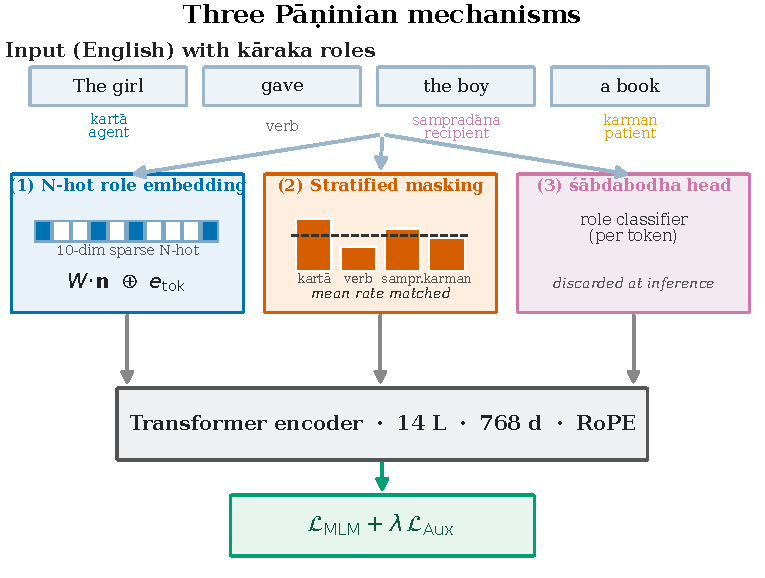
\includegraphics[width=\linewidth]{figures/fig_mechanism.pdf}
\caption{The three P\=a\d{n}inian mechanisms. (1) A Vidyut N-hot morpheme/role vector is projected and added to each token embedding; (2) k\=araka role-stratified masking sets per-role mask probabilities whose mean is budget-matched to the uniform baseline; (3) a \'s\=abdabodha auxiliary head predicts roles from the encoder hidden state and is discarded at inference. The encoder is trained with $\mathcal{L}_{\text{MLM}} + \lambda\,\mathcal{L}_{\text{aux}}$.}
\label{fig:mechanism}\end{figure}

For each token, Vidyut \cite{Prasad2024Vidyut} produces a morpheme-boundary annotation and a k\=araka-role label (kart\=a, karman, kara\d{n}a, samprad\=ana, ap\=ad\=ana, adhikara\d{n}a, or a separator class). A sparse binary 10-dimensional vector encodes these and is projected to 768 dimensions and added to the token embedding, requiring no architectural change. The masking strategy adapts by role, $p_{\text{mask}}(t) = \alpha\,p_{\text{base}} + (1-\alpha)\,p_{\text{role}}(r(t))$, with per-role probabilities rescaled to hold the mean mask rate constant, so any effect is attributable to the \emph{distribution} of masked tokens across roles rather than to total masked volume. The auxiliary objective predicts k\=araka roles via a token-level head combined with the MLM loss at weight $\lambda$ (typically 1.0) and discarded before evaluation.

Two objectives are compared: a hybrid MLM\,+\,CLM configuration (15\% masked, plus a causal next-token head weighted 0.5) and a pure-MLM configuration (CLM head removed). All models are evaluated on the official BabyLM suite: BLiMP \cite{Warstadt2020BLiMP} (67 minimal-pair paradigms), BLiMP Supplement, EWoK \cite{Ivanova2024EWoK}, Entity Tracking, COMPS \cite{Misra2023COMPS}, and GLUE \cite{Wang2019GLUE}. Reported results are means with 95\% confidence intervals over three to five seeds (single seed for exploratory 100M arms); arm comparisons use paired bootstrap over per-paradigm subsets with Holm--Bonferroni correction. The Strict baseline is 74.53 BLiMP and Strict-Small 65.08 \cite{Hu2024BabyLM}. Corpus, training stages, and full hyperparameters are in Appendices~\ref{app:data} and~\ref{app:train}.

\section{Results}
\label{sec:results}
We report three pre-registered findings: F1 (a scale-dependent objective effect, our principal positive), F2 (k\=araka masking at matched budget), and F3 (a k\=araka auxiliary objective over five seeds). Figure~\ref{fig:forest} places all four pre-registered effects on a common axis. Table~\ref{tab:official} situates both submission models on the official BabyLM~2026 leaderboard harness against the official baselines.

\begin{figure}[t]\centering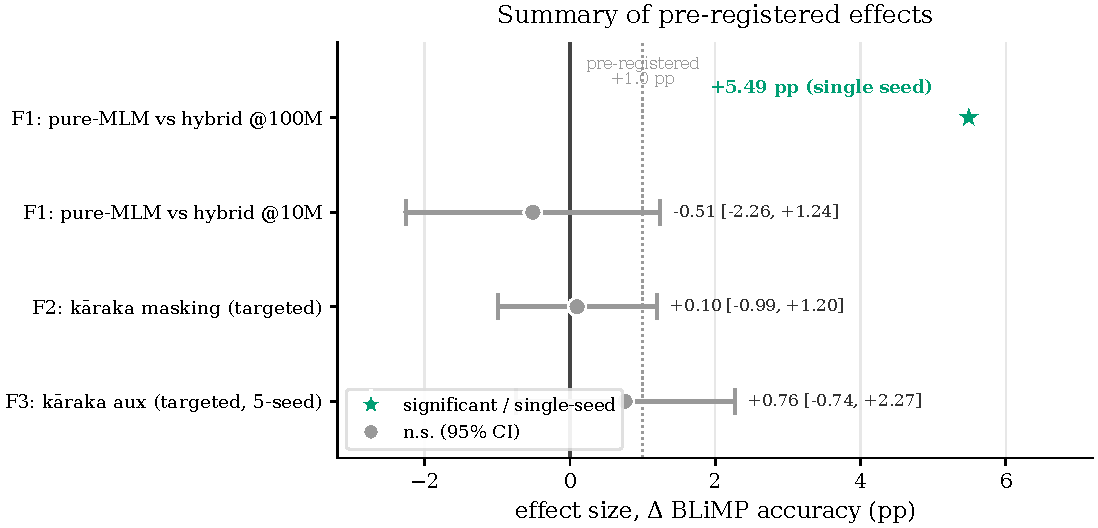
\includegraphics[width=0.92\linewidth]{figures/fig_findings_forest.pdf}
\caption{Summary of pre-registered effects on BLiMP (points). The 100M objective effect (F1) is the one large, robust positive; the 10M objective contrast and both k\=araka mechanisms fall within noise of the $+1.0$-point threshold (dashed). Whiskers are 95\% intervals; the 100M point is single-seed.}
\label{fig:forest}\end{figure}

\begin{table}[t]
\centering\small
\caption{Official BabyLM~2026 pipeline (the leaderboard harness) for both submission models against the official baselines \cite{Hu2024BabyLM}; per-task GLUE in Appendix~\ref{app:repro}. Our internal development harness scores the same checkpoints $\sim$5--6 points higher (73.06 / 64.09 BLiMP), a systematic offset (\S\ref{subsec:harness}).}
\label{tab:official}
\begin{tabular}{lcccc}
\toprule
 & \multicolumn{2}{c}{Strict (100M)} & \multicolumn{2}{c}{Strict-Small} \\
\cmidrule(lr){2-3}\cmidrule(lr){4-5}
Task & ours & base & ours & base \\
\midrule
BLiMP & 67.56 & 74.53 & 59.46 & 65.08 \\
BLiMP Suppl. & 63.81 & 65.00 & 55.08 & 57.25 \\
COMPS & 53.78 & 55.85 & 50.99 & 51.81 \\
EWoK & 52.35 & --- & 52.24 & --- \\
Entity Tracking & 22.28 & 23.58 & --- & 21.07 \\
GLUE (macro) & 63.28 & --- & 63.09 & --- \\
\bottomrule
\end{tabular}
\end{table}

\subsection{F1: Scale-Dependent Objective Effect}
A hybrid objective adds a causal language-modelling (CLM) head to the MLM loss, which may stabilize learning when the MLM signal is sparse but dilute it once MLM is strong. Pure-MLM and hybrid models are trained identically except for the objective, with three seeds at 10M tokens and single seeds at 100M. At 10M, pure-MLM achieves a 3-seed mean of 63.58 (95\% CI $\pm$1.73) versus hybrid 64.09 ($\pm$0.26), with overlapping intervals. At 100M, pure-MLM reaches 73.06 against hybrid 67.57, a 5.49-point advantage (Figure~\ref{fig:objscale}; internal harness). The CLM head's regularizing effect at 10M becomes a bottleneck at the larger budget. This speaks directly to GPT-BERT \cite{CharpentierSamuel2024}, whose hybrid masked-plus-causal training won BabyLM~2024: the hybrid recipe is not uniformly preferable, and at 100M tokens pure-MLM is the stronger choice on BLiMP. The 10M neutrality justifies retaining hybrid for the Strict-Small submission; the 100M result drives the Strict-track model.

\begin{figure}[t]\centering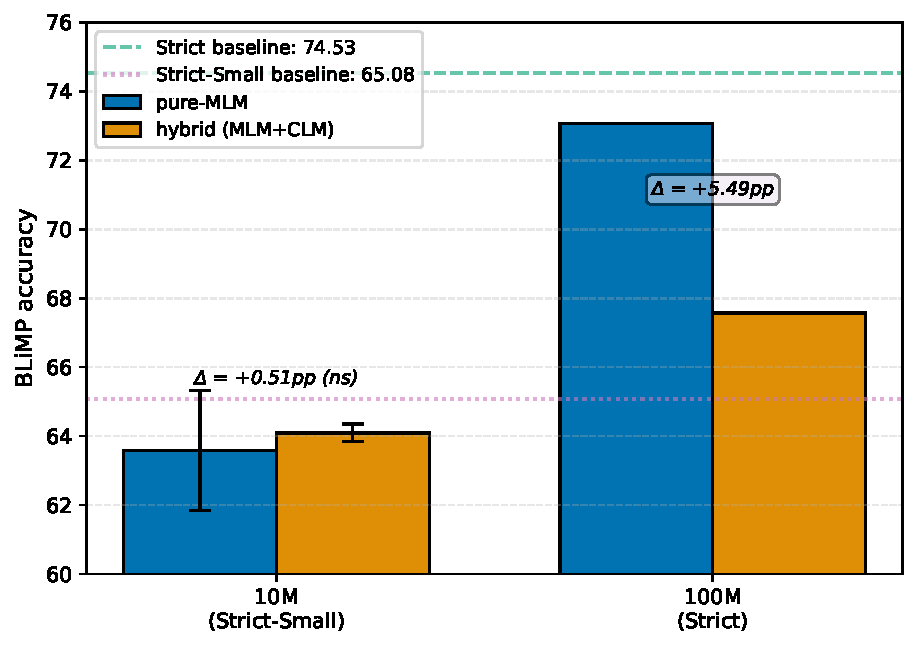
\includegraphics[width=0.82\linewidth]{figures/fig_objective_scale.pdf}
\caption{F1: pure-MLM versus hybrid MLM\texttt{+}CLM across the 10M- and 100M-token budgets (internal harness).}
\label{fig:objscale}\end{figure}

\paragraph{Training-seed sensitivity at 100M.}
We report the 100M figures as single-seed estimates. Re-running the locked recipe from identical initialization under two further seeds does not recover 73.06: best masked-LM losses of 1.61 / 1.82 (versus the submission seed's 0.515) and BLiMP of 58.3 / 53.6, with one optimizer trajectory diverging (Figure~\ref{fig:seeddiv}). Because initialization is held fixed, all trajectories begin identically and separate only during optimization; the evaluation is not implicated (the submission checkpoint re-evaluates to 73.06 and an independent pseudo-log-likelihood proxy reproduces all three scores within 0.4 points). The 100M recipe is thus not yet robust to the training seed: 73.06 is a valid but fortunate-seed outcome, and the magnitude of the 100M advantage is seed-sensitive. Stabilizing the recipe (gradient clipping, optimizer warmup, best-of-$N$) is future work.

\begin{figure}[t]\centering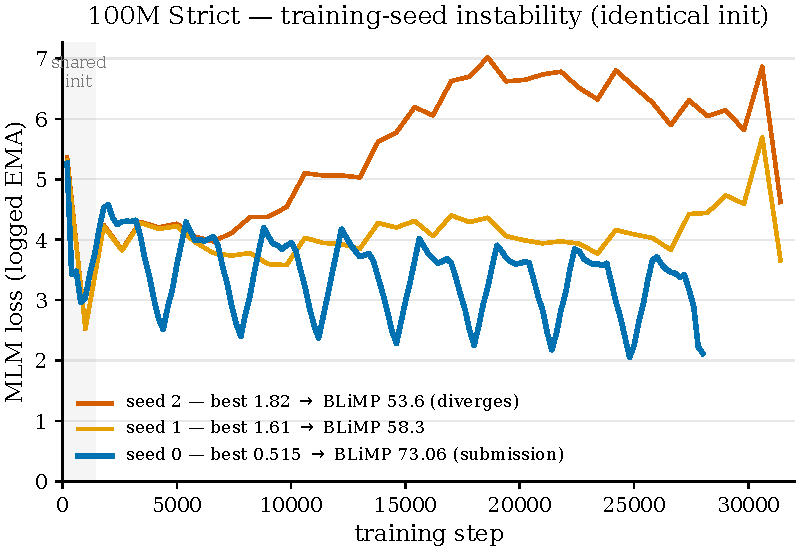
\includegraphics[width=0.92\linewidth]{figures/fig_seed_divergence.pdf}
\caption{Training-seed instability of the 100M recipe. All three seeds share an identical initialization (shaded) and begin together, then diverge: seed~0 (the submission) descends to the basin scoring 73.06, while seeds~1--2 plateau or climb and score 58.3 / 53.6.}
\label{fig:seeddiv}\end{figure}

\subsection{F2: K\=araka-Masking Causality (Matched Budget)}
K\=araka role-stratified masking (Arm K) is compared to uniform masking (Arm C) at identical mask budget (100M tokens, $n=1$ per arm), holding N-hot embeddings, RoPE, and pure-MLM fixed and disabling frequency-weighted masking ($\alpha=0$). The pre-registered primary metric is a paired bootstrap over 20 targeted paradigms. Arm K achieves 71.77 full / 82.03 targeted BLiMP; Arm C achieves 70.49 / 81.93. The targeted contrast is $\Delta_{K-C}=+0.10$ points (95\% CI $[-0.99,+1.20]$), not significant. Earlier exploratory runs reported a $+1.23$-point gain, but that reflected unmatched mask rates and frequency weighting; with matching enforced, the role distribution contributes no signal. F2 is a pre-registered null.

\subsection{F3: K\=araka Auxiliary Objective (5-Seed $t$-Test)}
The supervised k\=araka-role head is applied at 10M tokens ($\lambda=1.0$ versus $\lambda=0.0$), with corpus, hybrid objective, uniform masking, and seed list fixed. The pre-registered primary metric is the per-seed targeted delta. The 5-seed targeted mean is auxiliary 74.02 versus baseline 73.26 ($+0.76$ points, 95\% CI $[-0.74,+2.27]$; $t=1.41$, df\,=\,4, n.s.), attenuating from $+2.65$ at one seed to $+0.76$ at five, so the seed-0 result was seed luck. A specificity control sharpens this: a shuffled-role auxiliary (3-seed targeted mean 73.53) does \emph{not} reproduce the real-auxiliary effect (74.41), ruling out generic multi-task regularization and consistent with a weak, k\=araka-specific signal that is underpowered at 10M.

\subsection{Two Harnesses, and the Gap Between Them}
\label{subsec:harness}
All controlled comparisons above use a single internal masked pseudo-log-likelihood harness applied identically to every arm. The official BabyLM~2026 pipeline (Table~\ref{tab:official}) places the same checkpoints $\sim$5--6 points lower (67.56 versus 73.06 BLiMP for Strict; 59.46 versus 64.09 for Strict-Small). Both harnesses load the identical public checkpoints and the offset is systematic, so this is a scoring-convention difference, not a model difference, and it leaves the relative F1--F3 conclusions intact (they are within-harness contrasts). We report the official numbers as the leaderboard record and use the internal harness only for relative comparison. The methodological lesson: a model-selection harness must be calibrated against the scoring harness of record, or absolute claims will not transfer.

\section{Discussion and Conclusion}
\label{sec:discussion}
The robust gains localize to two architectural sources: positional encoding via RoPE and the choice of pretraining objective, whose effect is markedly scale-dependent (neutral at 10M, a 5.49-point pure-MLM advantage at 100M on the internal harness). In contrast, the k\=araka mechanisms carry no measurable causal weight on standard linguistic diagnostics: role-stratified masking is statistically indistinguishable from uniform masking at matched budget (the earlier apparent gain traced to mask-rate confounds), and the auxiliary's five-seed mean attenuates toward zero while resisting a shuffled-role control. These nulls do not falsify the hypothesis that argument structure matters for pretraining; they narrow scope, showing the specific mechanisms tested do not help at the 10M--100M-token budget on English BLiMP. Larger models, longer training, multilingual settings, or compositional-generalization benchmarks (COGS, SCAN, CFQ) may behave differently.

The value is methodological as much as empirical: pre-registration with effect-size thresholds, matched-budget controls that eliminate the mask-rate confound, multi-seed validation that exposes inter-seed variance, and transparent reporting of nulls, of training-seed instability at 100M, and of a systematic evaluation-harness offset. Two cautions stand out for the field: a single fortunate seed can masquerade as a robust result at 100M, and a model-selection harness that is not calibrated to the scoring harness of record will overstate absolute performance. Both are reported here in full. Code, checkpoints, and the official-pipeline prediction files are released (anonymized for review).

\bibliography{references_new}

\appendix

\section{Architecture and Training Configuration}
\label{app:train}
Both tracks use a 14-layer Transformer encoder (hidden 768, 12 heads, feed-forward 3072) with RoPE positional encoding and the Muon (Newton--Schulz orthogonalized momentum) optimizer at peak learning rate $1\times10^{-3}$ with cosine annealing and 5\% linear warmup. Batch size is 256 sequences of length up to 192; the masking rate follows a cosine schedule from 0.40 to 0.15 over 10 epochs. The tokenizer is a 20{,}000-piece SentencePiece BPE built jointly over English and Sanskrit. The Strict model ($\sim$100M parameters, 100M-token budget) and Strict-Small model ($\sim$114M parameters, 10M-token budget) are trained on a single 128\,GB unified-memory accelerator; a 100M-token run takes $\approx$13.7 hours and a 10M-token run $\approx$82 minutes. The N-hot projection $W\in\mathbb{R}^{768\times10}$ maps the sparse role vector to the hidden dimension and is added to the token embedding before encoding; the auxiliary head is a token-level role classifier trained with weight $\lambda$ and discarded at inference.

\section{Corpus, Curriculum, and Dose Arms}
\label{app:data}
Pretraining uses the official BabyLM Strict (100M words) and Strict-Small (10M words) English corpora mixed with a small in-budget Sanskrit component from the Digital Corpus of Sanskrit and GRETIL, plus a synthetic P\=a\d{n}inian dose generated by the Vidyut-Praky\=a derivation engine; English comprises $\sim$95\% of tokens, and the total stays within the track word budget. Vidyut annotations (morpheme boundaries, k\=araka roles) are precomputed and cached for determinism. A frozen pre-pretraining dose ablation at 60M-token proxy scale compared Arm~A (English control), B (P\=a\d{n}inian), C (Dyck control), and D (Paribh\=a\d{s}\=a), scoring 64.15 / 63.54 / 63.85 / 63.77 BLiMP---a 0.61-point spread (null), so the dose was not used in the leaderboard submissions.

\section{Reproducibility and Per-Task Results}
\label{app:repro}
\paragraph{Locked recipe.} The validated 100M Strict submission was trained at the code state recorded under the commit message \emph{``LOCK pure-MLM for 100M Strict run.''} Recipe: objective MLM, dose-arm A with zero pre-pretraining epochs, ten English epochs, RoPE, N-hot embeddings, role-stratified masking (cosine 0.40$\to$0.15, frequency weight $\alpha=0.5$), max sequence length 192, vocabulary 20{,}000, Muon at peak LR $1\times10^{-3}$, seed 0; best loss 0.515. Re-running this recipe from identical initialization under two further seeds reaches best losses 1.61 / 1.82 and BLiMP 58.3 / 53.6 (Table~\ref{tab:seedrepro}); the divergence is a training-seed instability the seeding exposed, not an evaluation error (the checkpoint re-evaluates to 73.06 on the official pipeline, and an independent proxy reproduces all three scores within 0.4 points). Code, checkpoints, and official prediction files are released (anonymized for review).

\begin{table}[h]
\centering\small
\caption{Training-seed sensitivity of the 100M recipe (identical initialization).}
\label{tab:seedrepro}
\begin{tabular}{lcc}
\toprule
Seed & best MLM loss & BLiMP \\
\midrule
0 (submission) & 0.515 & 73.06 \\
1 & 1.61 & 58.3 \\
2 & 1.82 & 53.6 \\
\bottomrule
\end{tabular}
\end{table}

\paragraph{Official per-task GLUE.} Table~\ref{tab:official_glue} reports the official-pipeline GLUE results (zero-shot results are in Table~\ref{tab:official}).

\begin{table}[h]
\centering\small
\caption{Official 2026-pipeline GLUE (accuracy, except MRPC/QQP F1) for both submission models, with baselines where reported.}
\label{tab:official_glue}
\begin{tabular}{lcccc}
\toprule
Task & Strict & base & S-Small & base \\
\midrule
BoolQ & 67.03 & 67.46 & 65.99 & 65.87 \\
MNLI & 48.84 & 59.94 & 46.37 & 49.80 \\
MRPC & 82.04 & 84.35 & 82.57 & 83.49 \\
MultiRC & 57.55 & 63.90 & 57.88 & 64.52 \\
QQP & 64.83 & 70.73 & 63.03 & 60.86 \\
RTE & 61.15 & 56.83 & 60.43 & 60.43 \\
WSC & 61.54 & --- & 65.38 & --- \\
\midrule
Macro & 63.28 & --- & 63.09 & --- \\
\bottomrule
\end{tabular}
\end{table}

\paragraph{F1/F3 per-seed (internal harness).} F1 10M pure-MLM seeds: 65.22 / 63.31 / 62.20 (mean 63.58); hybrid 3-seed mean 64.09 ($\pm$0.26). F3 targeted per-seed deltas: $+2.65, +0.61, +1.12, -0.22, -0.34$ (5-seed mean $+0.76$, $t=1.41$, df\,=\,4, n.s.).

\end{document}
